\documentclass[12pt,letterpaper]{article}
\usepackage{fullpage}
\usepackage[top=2cm, bottom=4.5cm, left=2.5cm, right=2.5cm]{geometry}
\usepackage{amsmath,amsthm,amsfonts,amssymb,amscd}
\usepackage{lastpage}
\usepackage{enumerate}
\usepackage{fancyhdr}
\usepackage{mathrsfs}
\usepackage{xcolor}
\usepackage{graphicx}
\usepackage{listings}
\usepackage{hyperref}
\usepackage{amsmath}
\usepackage{mathtools}
\usepackage{tikz}
\usepackage{array}
\usetikzlibrary{matrix}

\hypersetup{%
  colorlinks=true,
  linkcolor=blue,
  linkbordercolor={0 0 1}
}
 
\renewcommand\lstlistingname{Section}
\renewcommand\lstlistlistingname{Algorithms}
\def\lstlistingautorefname{Alg.}

\lstdefinestyle{Python}{
    language        = Python,
    frame           = lines, 
    basicstyle      = \footnotesize,
    keywordstyle    = \color{blue},
    stringstyle     = \color{green},
    commentstyle    = \color{red}\ttfamily
}

\setlength{\parindent}{0.0in}
\setlength{\parskip}{0.05in}

% Edit these as appropriate
\newcommand\course{CSE 3500}
\newcommand\hwnumber{6}                  % <-- homework number
\newcommand\NetIDa{rjf23002}           % <-- NetID of person #1
\newcommand\NetIDb{}           % <-- NetID of person #2 (Comment this line out for problem sets)

\pagestyle{fancyplain}
\headheight 35pt
\lhead{\NetIDa}
\lhead{\NetIDa\\\NetIDb}                 % <-- Comment this line out for problem sets (make sure you are person #1)
\chead{\textbf{\Large Homework \hwnumber}}
\rhead{\course \\ \today}
\lfoot{}
\cfoot{}
\rfoot{\small\thepage}
\headsep 1.5em

\begin{document}

\section*{Problem 0}
\begin{enumerate}
  \item
    3 cases: \\
    Case 1: if P == 10K: Bring either \\
    Case 2: if P $>$ 10K: Bring 4 pineapples \\
    Case 3: if P $<$ 10K: Bring 40 kiwis \\

    We could potentially map the variables using equations to form linear equations.
    For example, we choose to bring n kiwis and m pineapples.
    To minimize the difference in happiness,
    we should ideally bring an amount where nP = mK is satisfied.
    Additionally, by the weight constraint, we should bring an amount
    that satisfies nk + mp = c, where capacity c = 40k = 4p, where k and p
    are weights of a single kiwi and pineapple respectively. \\

    But given the fact that we do not know the true value of either of these variables, 
    the best strategy in this case would be to spend 50\%, or half of our
    capacity, on kiwis and the rest on pineapples.
    Hence, we would bring 20 kiwis and 2 pineapples.
  \item
    Case 1:  \\
    The oracle would choose to bring 40 kiwis to get a happiness value of 40K.
    We would get a happiness value of 40K as well. \\
    Case 2: \\
    The oracle would choose to bring 4 pineapples to get a happiness value of 4P.
    We would get a happiness value of 20K + 2P $<$ 4P. \\
    Case 3: \\
    The oracle would choose to bring 40 kiwis to get a happiness value of 40K.
    We would get a happiness value of 20K + 2P $<$ 40K. \\\\
    Thus, we have the competitive ratios of 1, $\frac{P}{10K}$ $>$ 1, $\frac{K}{10P}$ $>$ 1,
    and hence the possible maximum value is 
    max($\frac{P}{10K}$, $\frac{K}{10P}$) depending on the values of P and K.
  \item
    By the previous parts, \\
    Opt(P, K) = $n_{k}$*K + $n_{p}$*P
    where $n_{k} * w_{k}$ + $n_{p} * w_{p}$ $\leq$ c, \\
    where c = 40 * $w_{k}$ = 4 * $w_{p}$ and 10 * $w_{k}$ = $w_{p}$
  \item
    When $n_{k}$ = 20 and $n_{p}$ = 2, say in the extreme case that 
    Professor Derek really hates pineapples such that the joy value he gets out of it is P = 0.
    In that case, the oracle would bring 40 kiwis instead, providing him with a joy value of 40K.
    Meanwhile, we can only provide him with a joy value of 20K.
    As such, we have a competitive ratio of 2.
    As this value is only one of the maximum values, we can say that the
    competitive ratio is at least 2.
  \item
    \begin{enumerate}[a)]
      \item
        When K = 0 and P = 0, whatever combination of kiwis and pineapples will always
        land us with an arbitrary constant joy value of x.
        This is because even if we increase or decrease any amount of fruits that we bring, 
        it does not change the final joy value that we can gain of x.
        As such, the oracle would try to choose a desirable combination,
        but only bring about x amount of joy.
        On the other hand, whatever decision we make, we also only bring about x amount of joy.
        Hence, the competitive ratio here would be 1 in all cases, and is thus upper bounded by 2.
      \item 
        Using the claim, let us take the case of P $>$ K as case 1.
        The oracle would thus take 4P while we take 20K + 2P.
        As 20K is equivalent to 2P, and since P $>$ 0, our competitive ratio is $\frac{4P}{2P < n < 4P}$,
        where the joy value will thus be a number between 1 and 2. 
        Hence, we can say it is upper bounded by 2. \\
        Let us take the case of K $>$ P as case 2.
        The oracle would thus take 40K while we take 20K + 2P.
        As 2P is equivalent to 20K, and since K $>$ 0, our competitive ratio is $\frac{40K}{20K < n < 40K}$,
        where the joy value will thus be a number between 1 and 2. 
        Hence, we can say it is upper bounded by 2.
      \item
        Under this combination of gifts, we can't go horribly wrong as our 
        choice could be only at most 2x worse than the optimal.
        However, if we manage to predict well, we would be able to offer Professor Derek a high amount of joy.
    \end{enumerate}
\end{enumerate}

\newpage

\section*{Problem 1}
Algorithm:
Given weight $w_{i}$ and value $v_{i}$ of an arbitrary doll, we can calculate $d_{i}$,
where we let $d_{i}$ = $\frac{v_{i}}{w_{i}}$.
Essentially, $d_{i}$ represents the value a doll gives per unit weight. 
After calculating all these values, we can sort it in descending order.
From there, we greedily take the doll that has the highest d value, 
up till we run out of capacity, or if we have taken the whole doll.
If we run out of capacity, we can always decompose the doll and take a fraction of it.
If we have taken the whole doll and we still have remaining capacity, 
then we can go down the next item in the list and repeat this process.
We continue this until we either run out of dolls to choose from or we reached our capacity. \\

Correctness: 
Let us assume that we have made choices $c_{0}, c_{1}, ..., c_{i - 1}$
such that choice $c_{i}$ veers off from the optimal solution.
We assume that choices $c_{0}$ to $c_{i - 1}$ are optimal choices such that they maximize the value as per the question.
Let us take a look at choice $c_{i}$.
For the $i^{th}$ choice, our algorithm takes the doll which can provide us
with the greatest d value (doll value per unit weight).
Suppose the optimal solution also chose this, 
that would be trivial and it would lead to the same result.
However, suppose that this is not the case.
Pausing the algorithm at $c_{i - 1}$, we see that we likely have some arbitrary amount of capacity m.
The next best option may seemingly be to fill it in with the doll that gives us the largest value v,
however that might not be beneficial in terms of weight efficiency.
Instead, it would be more beneficial to choose the next doll based on its value over per unit weight,
to get the doll with the highest weight efficiency to maximize our remaining capacity.
So we have come up with a new decision scheme, that is at least as good as the 
purported optimal solution but does include our decision.

\newpage

\section*{Problem 2}

\begin{figure}[!h]
  \centering
  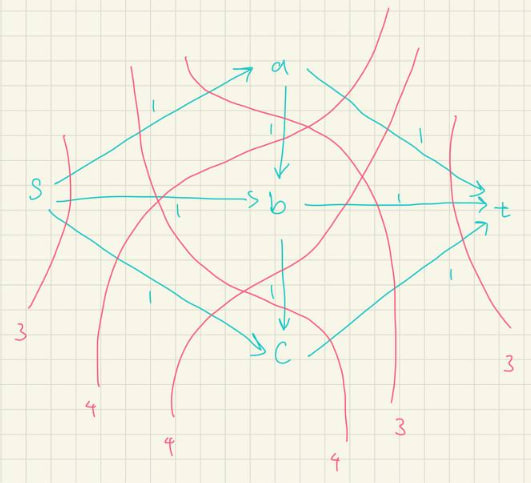
\includegraphics[width=0.9\linewidth]{q2.1.jpg}
  \caption{Min cuts for graph 1}
  \end{figure}

\newpage

\begin{figure}[!h]
  \centering
  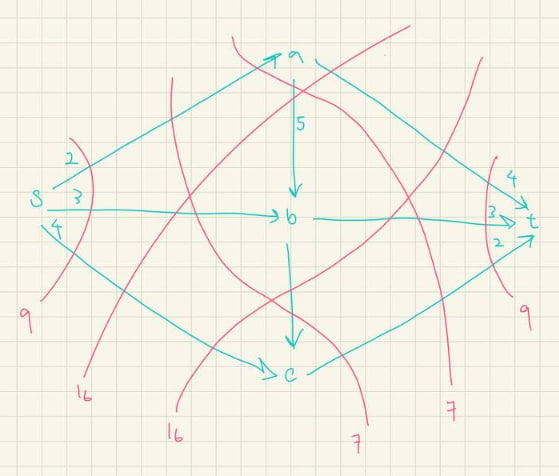
\includegraphics[width=0.9\linewidth]{q2.2.jpg}
  \caption{Min cuts for graph 2}
  \end{figure}

\newpage

\section*{Problem 3}

\begin{enumerate}
  \item 
    \begin{figure}[!h]
      \centering
      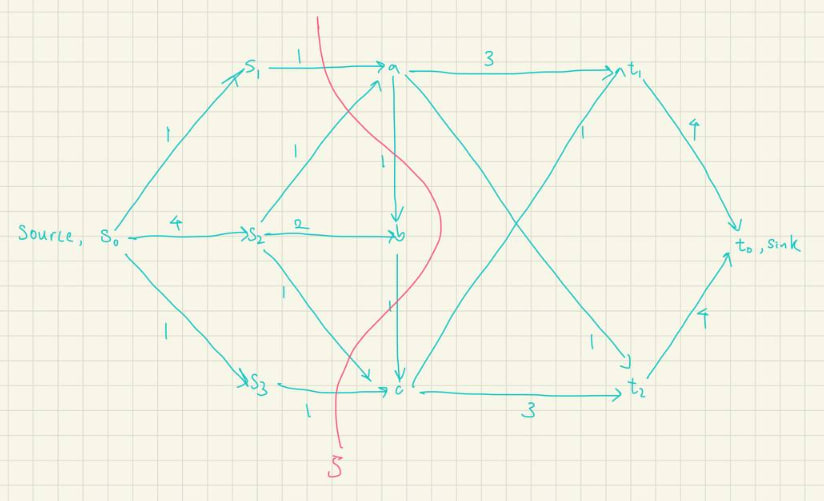
\includegraphics[width=0.9\linewidth]{q3.1.jpg}
      \caption{Modified Flow Graph}
      \end{figure}
      
    For this problem, we can modified the flow graph such that it can be solved with the 
    single source Ford-Fulkerson algorithm.
    As the initial problem involves multiple sources and multiple sinks, 
    we can augment the problem to have only a single source and single sink by
    adding a supersource and supersink.
    The supernodes branch out to the respective sources and sinks.
    The capacities on each new edge would thus be equal to the sum of the outgoing edges from
    the sources and the incoming edges from the sink for each respective node.
    Thus, this does not change anything fundamentally about the graph as well as its capacities,
    but allows us to run single source Ford-Fulkerson to solve this problem.
    Thus, we can run the algorith or find the minimum cut to yield us
    the maximum flow to this problem, which would be 5.
  \item 
    Let us say that there are r residents and h hospitals such that r $\leq$ h.
    This ensures us that each resident can be matched to at least a h.
    We also make the assumption that every h has at least one in-degree of 1, 
    signifying that it is at least preferred by some resident r regardless of its priority.
    Lastly, we assume that each hospital can only accommodate up to 1 resident. \\
    
    Since each resident has 3 choices, let us keep a hashmap of residents and their choices.
    The keys shall be the resident $r_{i}$ with the values being a list of choices in descending order.
    Now, we can form a bipartite graph using our residents r having directed edges to our hospitals h.
    We take the idea from the previous part, creating supernodes for the source and sink belonging
    to the residents and hospitals respectively.
    We however subject the capacity of every single edge to be 1, 
    this allows us to ensure that each hospital can only be picked once.
    We can also use another hashmap to store the available capacity for each edge. 
    With this, we have our flow graph.
    To solve this question, an algorithm we can apply is to pick an unassigned resident r at random,
    and enumerate his choices by checking the hashmap.
    We pick the first available choice, and update the capacity to indicate that the hospital is taken.
    We can then repeat this until all residents are assigned.
    This algorithm ensures that each resident is at least matched to a hospital of their 3 choices,
    due to our earlier assumptions stated in the first paragraph.
\end{enumerate}

\end{document}
